\begin{figure}[!ht]
    \centering
    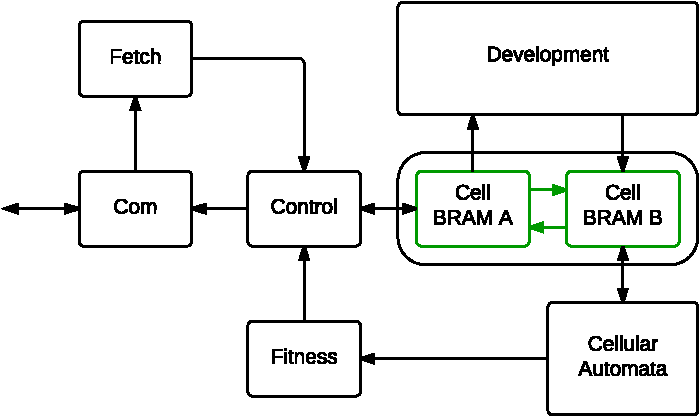
\includegraphics[width=0.8\textwidth]{implementation-simple}
    \caption[High-level system diagram]{High-level block diagram of the new hardware platform.}
    \label{fig:implementation-simple}
\end{figure}

\begin{sidewaysfigure}[!pt]
    \centering
    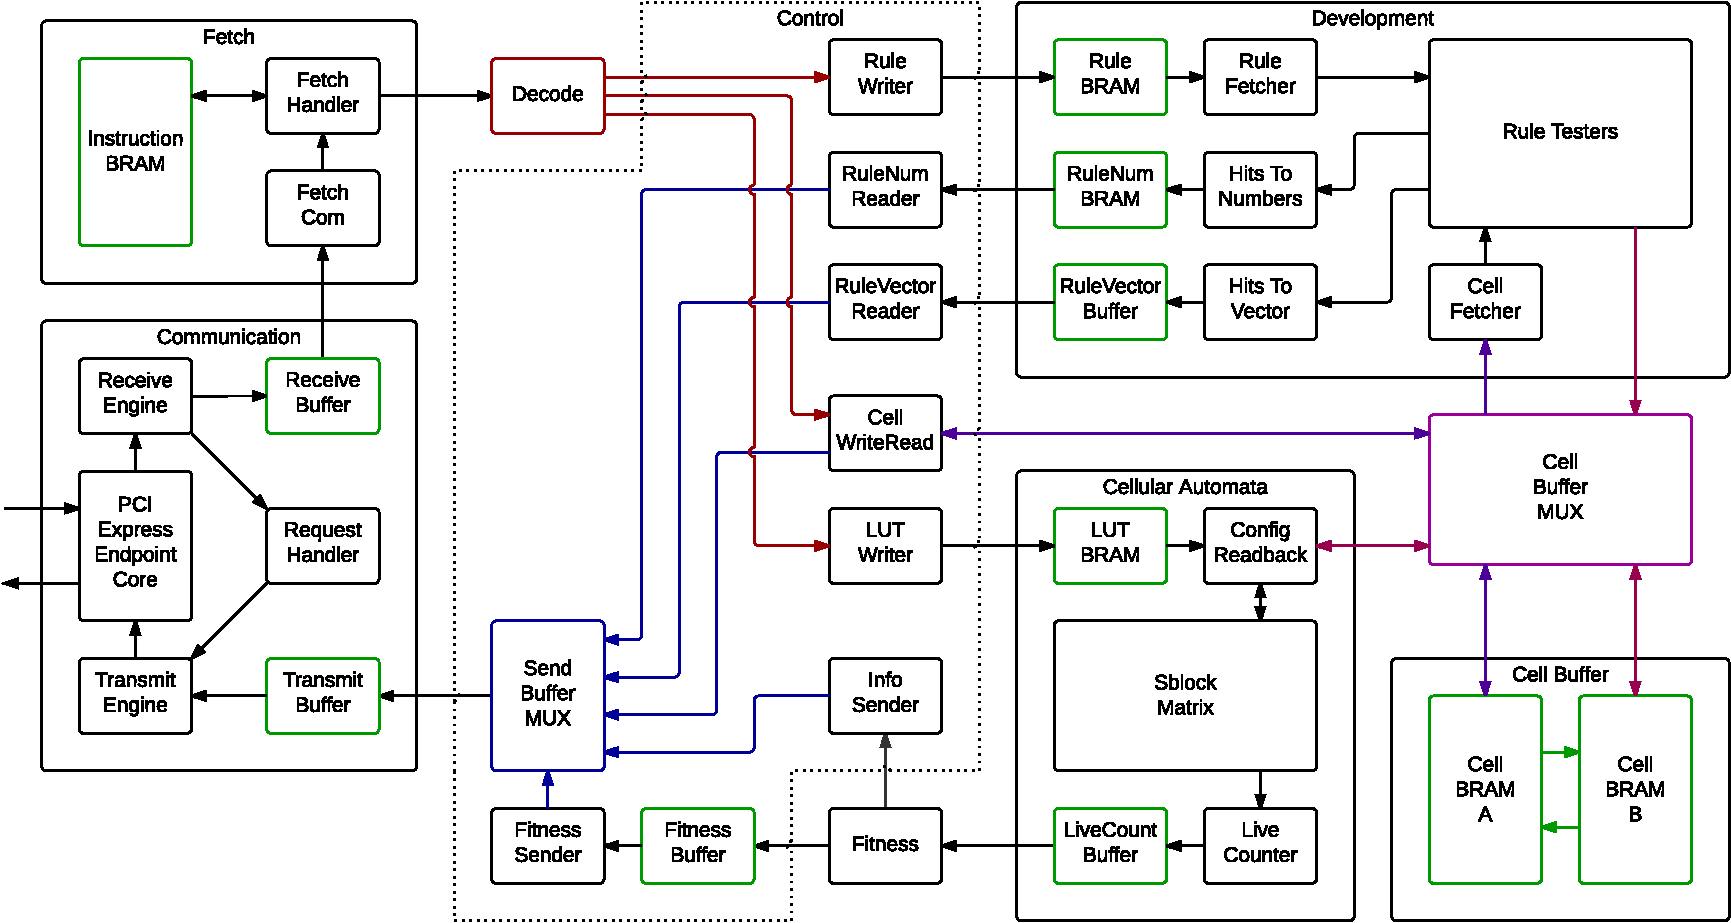
\includegraphics[width=\textwidth]{implementation-full}
    \caption[Detailed system diagram]{
        Detailed block diagram of the new hardware platform.
        Control is implemented as a group of modules, marked by a dotted border.
        Some signals are color-coded for increased readability.
        Signals from Decode are colored red, while those to the Send and Cell Buffer Multiplexers are colored blue and purple respectively.
        Note the two different hues of purple for the different Cell BRAMs.
        Control signals are not shown.
    }
    \label{fig:implementation-full}
\end{sidewaysfigure}

The platform is design as an interlocked pipeline.
The main stages are Fetch, Decode and Execute, but due to interlocking, each stage can contain sub-pipelines or state machines.

The Execute stage is special in that is is split into many sub-modules, where only one is activated at a time.
The exception is Fitness, which is always active, since it operates in a dataflow-like fashion.
A hazard detection unit could be implemented to increase performance by allowing multiple non-conflicting units run in parallell.

Interlocking is implmented using special Run and Done signals.
Run is asserted when all modules asserts Done.

All state machines are of Mealy design with clocked output, unless noted otherwise.

\todo{Rewrite this!}

%==============================================================================%

\section{General Consepts}

\todo{Control signals not shown, only data}
\todo{Borders: Green = BRAM, grey = outside}
\todo{BRAM vs Buffer. Move buffer description here?}

\subsection{Parameterization}

\begin{itemize}
    \item Used pretty much everywhere
    \item Most can be 1 to inf
    \item Asserts where restrictions apply
    \item List them all?
\end{itemize}

\subsection{Pipelining}

The new hardware design makes extensive use of pipelining, and since many stages use a variable amount of cycles for a variety of reasons \todo{which? state machine, pipeline in pipeline, simpler}, interlocking is used in nearly all pipelines.
Interlocking is implemented with two signals connected to each stage: Run and Done.
When a stage does not require further cycles to finish, it asserts its Done signal and then waits for the Run signal before continuing.
The Run signals for all stages are asserted when all Done signals are asserted.
Each stage then resets its Done signal and the process repeats.
An example is shown in \figurename~\ref{fig:wavediagram-pipeline}.

\begin{figure}[!ht]
    \centering
    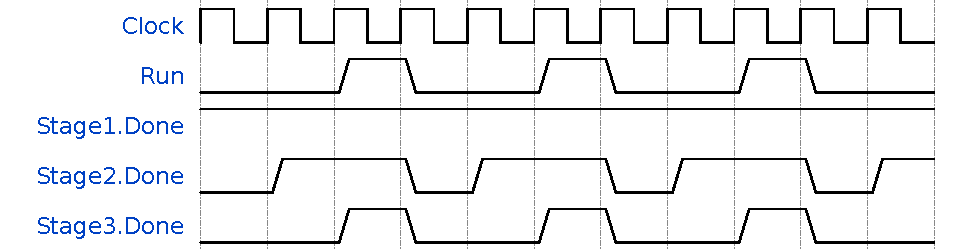
\includegraphics[width=0.9\textwidth]{wavediagram-pipeline}
    \caption[Pipeline wave diagram]{
        Wave diagram showing pipeline interlocking signals for a 3-stage pipeline where the stages complete in one, two and three cycles respectively.
    }
    \label{fig:wavediagram-pipeline}
\end{figure}

Often, a multi-cycle stage only looks at its input in the first cycle to determine its execution path.
This can be taken advantage of to reduce register usage by ruling that the data in the pipeline registers only have to be valid when Run is asserted.
The stages can then write directly to their output registers, instead of caching partial output internally in extra registers.
If a stage happens to require the output of the previous stage for multiple cycles however, input caching is needed.
This causes no register usage reduction in the worst case, while the register usage is halved in the best case.
The common case for this design is to only look at the input the first cycle for most signals, which should provide a nice reduction.

\subsection{Buffers}

All buffers are implemented as first-in first-out (FIFO) queues using block RAM (BRAM) and two counters.
The counters determine the addresses that are written to and read from, and are incremented when the write or read signals are asserted.
\figurename~\ref{fig:wavediagram-fifo} shows how the FIFO is used to buffer two words.

\begin{figure}[!ht]
    \centering
    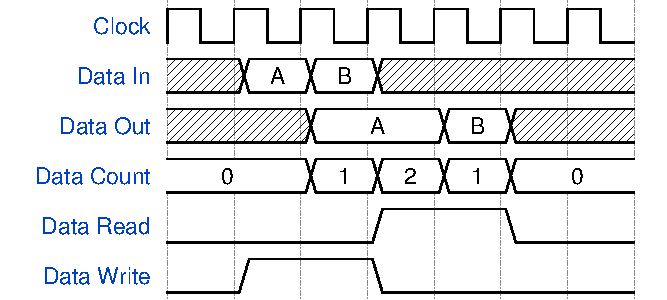
\includegraphics[width=0.7\textwidth]{figures/wavediagram-fifo}
    \caption[FIFO buffer wave diagram]{
        Wave diagram for the FIFO buffer, showing two consecutive writes followed by two consecutive reads.
    }
    \label{fig:wavediagram-fifo}
\end{figure}

Notice how the read signal needs to be asserted before the clock tick when data is read to ensure correct consecutive reads.
This is due to the BRAM used in the FIFO, which updates at clock ticks.
To have correct data available for a read in the following cycle, the address therefore has to be updated before the clock tick (by asserting the read signal).

%==============================================================================%

\section{Communication}

The new communication unit is based on Xilinx' reference PCI Express programmed input/output design.
It consists of the Xilinx PCI Express endpoint core, reception and transmission engines, data buffers, and a special request handler, as shown in \figurename~\ref{fig:implementation-communication}.

\begin{figure}[!ht]
    \centering
    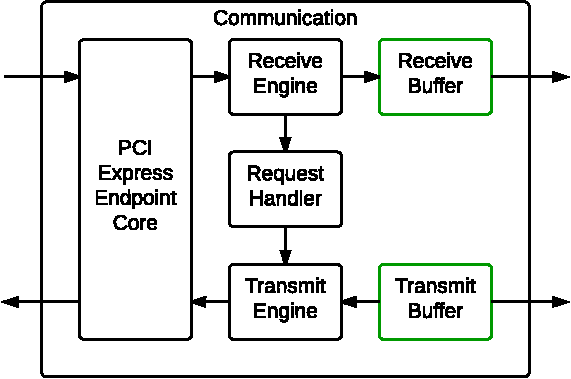
\includegraphics[width=0.7\textwidth]{implementation-communication}
    \caption[Communication module]{
        Detailed block diagram of the communication module.
    }
    \label{fig:implementation-communication}
\end{figure}

The endpoint core completely handles the physical and data link layers, and all TLPs related to configuration and establishment of the PCI Express connection.
Other TLPs, such as read and write requests, are presented on an AXI4-Stream interface \cite{ug672}.
The reception engine is responsible for parsing TLPs and either writing received data to the reception buffer or notifying the transmission engine about a read request.
The transmission engine is responsible for building completer TLPs to respond to read requests, using data from the transmission buffer.
The request handler listens to the read requests provided by the reception engine, and can override the transmission engine to respond to special requests.

\subsection{PCI Express Endpoint Core}

Several Spartan-6 FPGAs, including the one used in this project, contain a special-purpose hardware block for implementation of PCI Express.
The block completely handles the physical and data link layers, with the transaction layer left for the user.

To make use of the block, Xilinx provides the Spartan-6 Integrated PCI Express Endpoint Core; version 2.3 was used in this project.
This core additionally takes care of all TLPs related to configuration of the PCI Express connection.
Other TLPs, such as read and write requests, are presented on an AXI4-Stream interface \cite{ug672}.

The endpoint core is configured with two memory regions, both 4 kB in size\footnotemark.
\footnotetext{
    The smallest memory region that can be memory-mapped is one page. The default page size in Linux is 4 kB.
}
The first memory region (BAR0) is used for normal communication, while the second (BAR1) is used for special requests.
The separation is mostly conseptual as both regions are treated as one data stream.
The difference is that the special request handler kicks in for read requests to BAR1.

\subsection{Reception engine}

The reception engine is implemented as a simple state machine, as shown in \figurename~\ref{fig:statemachine-receive}.

\begin{figure}[!ht]
    \centering
    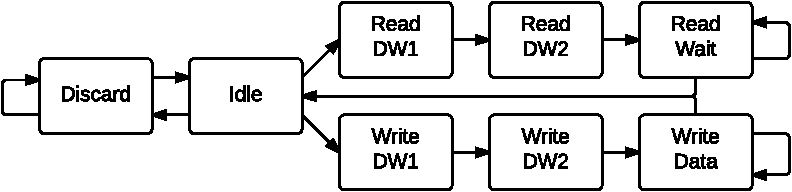
\includegraphics[width=0.8\textwidth]{statemachine-receive}
    \caption[Reception engine state machine]{
        State machine for the reception engine.
    }
    \label{fig:statemachine-receive}
\end{figure}

Until the endpoint core presents valid data, the state machine remains in Idle.
When it does, the data is stored, and the TLP type is checked.
If it is a read or write request, the state machine continues down the corresponding path, otherwise the remaining data is discarded.
The remaining portion of the TLP headers are then parsed in the DW1 and DW2 states.
For read requests, the state machine waits in ReadWait until the transmission engine is ready to accept a new read request, and then proceeds to Idle.
For write requests, the state machine stays in WriteData, where one DW of data is written to the reception buffer each cycle, for the length of the packet, and then proceeds to Idle.

\subsection{Transmission engine}

The transmission engine is implemented as a simple state machine, as shown in \figurename~\ref{fig:statemachine-transmit}.

\begin{figure}[!ht]
    \centering
    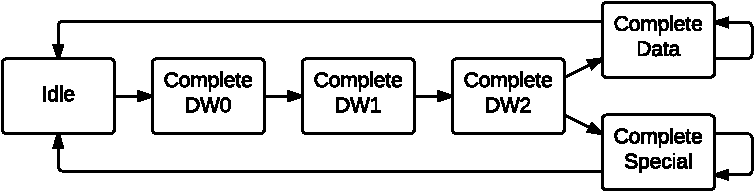
\includegraphics[width=0.8\textwidth]{statemachine-transmit}
    \caption[Transmission engine state machine]{
        State machine for the transmission engine.
    }
    \label{fig:statemachine-transmit}
\end{figure}

Until the reception engine signals a read request, the state machine remains in Idle.
When a read request is signaled by the reception engine, the state machine begins to traverse the DW path.
The DW0, DW1 and DW2 states each transmit one DW of the completer TLP header.
Then if the special request signal is set, it procceds to CompleteSpecial, where it transmits data presented by the request handler.
Otherwise, it proceeds to CompleteData where it transmits one DW of data from the transmission buffer each cycle.
When the requested number of DWs has been transmitted it proceeds back to Idle.

\subsection{Request handler}

The request handler continually listens to the read requests presented by the reception engine.
If the request is targeting the primary memory area (BAR 0), it is a normal read request and the transmission engine is allowed to proceed as usual.
Otherwise, it is a special request and the transmission engine is overridden.

The kind of special request is determined by the address of the read request, and handled thereafter.
There are currently four special requests implemented, as shown in Table~\ref{tab:requests}.

\begin{table}[!ht]
    \renewcommand{\arraystretch}{1.3}
    \centering
    \begin{tabular}{c|l}
        \bfseries Address & \bfseries Request \\
        \hline
        0x00 & Get transmission buffer data count \\
        0x01 & Get transmission buffer available space \\
        0x02 & Get reception buffer data count \\
        0x03 & Get reception buffer available space \\
    \end{tabular}
    \caption{Special requests.}
    \label{tab:requests}
\end{table}

Note that each of the implemented special requests assumes a read request length of one DW.
If the request has a greater length, the returned data is simply repeated to fill the packet.

%==============================================================================%

\section{Fetch}

The Fetch module is responsible for retrieving the next instruction that should be decoded and then executed.
It also handles all control flow.
It is implemented as a two-stage interlocked pipeline consisting of a Fetch Communication module and a Fetch Handler module connected to an Instruction BRAM.
This is shown in \figurename~\ref{fig:implementation-fetch}.

\begin{figure}[!ht]
    \centering
    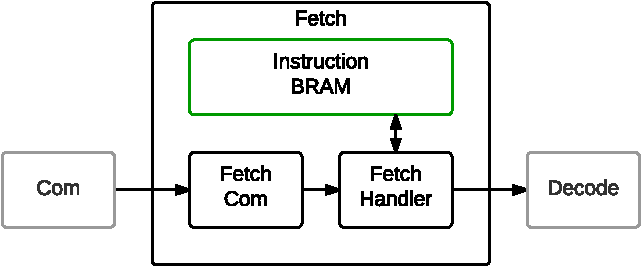
\includegraphics[width=0.7\textwidth]{implementation-fetch}
    \caption[Fetch module]{Detailed block diagram of the Fetch module.}
    \label{fig:implementation-fetch}
\end{figure}

Fetch Communication is responsible for converting data from the communication module into instructions while the Fetch Handler handles \todo{something that cover all operations}.
Both stages are implemented as state machines, making interlocking necessary.

\subsection{Fetch Communication}

While instructions are 256-bit, the communication interface is only 32-bit.
This means that the host system has to split each instruction into multiple 32-bit pieces.
As detailed in Appendix \todo{add ISA}, many instructions make use of less than 256 bits.
In fact, most instructions fit within the first 32 bits.
Sending all 256 bits for each instruction is therefore a bit excessive.
To optimize communication, the first 32-bit piece of each instruction has a field declaring the amount of following pieces required for reassembly.

The job of the Fetch Communication module is to combine all the pieces back into full 256-bit instructions.
It starts by reading the first 32-bit piece and setting all other bits to zero.
Then, the 3-bit instruction length field is analysed to determine how many further pieces are part of the same instruction.
The remaining pieces are then incorporated into the instruction, before it is passed on to the Fetch Handler.

\subsection{Fetch Handler}

The Fetch Handler has three modes of operation: FetchCom, FetchMem and StoreMem.
The modes and transitions are implemented as a state machine, which is shown in \figurename~\ref{fig:statemachine-fetch-handler}.

\begin{figure}[!ht]
    \centering
    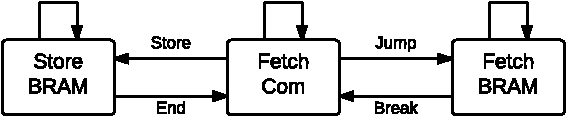
\includegraphics[width=0.6\textwidth]{statemachine-fetch-handler}
    \caption[Fetch Handler state machine]{State machine for the Fetch Handler.}
    \label{fig:statemachine-fetch-handler}
\end{figure}

In FetchCom mode, instructions are fetched from communication and sent to decode.
Since a variable-length format is used, this may take multiple cycles.
To make sure that instructions does not get "stuck" in the pipeline due to no further instructions arriving at the communication interface, NOPs are sent when Fetch Communication is busy.
When encountering a Store instruction, it enters StoreMem mode and for a Jump instructions it enters FetchMem mode.

In FetchMem mode, instructions are fetched from InstructionBRAM and sent to decode.
The first InstructionBRAM address is specified by the Jump instruction, and then it is incremented by one after each instruction.
When encountering a Break instruction, it enters FetchCom mode.

In StoreMem mode, instructions are fetched from communication and stored in InstructionBRAM.
The first InstructionBRAM address is specified by the Store instruction, and then it is incremented by one after each instruction.
Instructions are stored in full 256-bit format.
When encountering an End instruction, it enters FetchCom mode.

Control flow is implemented by having N M-bit general counters and a JumpEqual instruction.
The counters can be incremented or reset using special instructions.
The JumpEqual instruction is treated as a Jump instruction when the specified counter matches the specified value, otherwise it is discarded.

%==============================================================================%

\section{Decode}

Decode is responsible for parsing instructions, setting up control signals and passing instruction parameters to activated modules.
It is a very simple module, being essentially a giant switch statement with a case for each instruction.

Control signals are sent to all toplevel modules except communication, fetch and fitness.
\todo{why not fitness? dataflow-like}
By default, all modules are given a no-operation signal and multiplexers stay unchanged.
Then, depending on the instruction's operation code, the control signal for the appropriate module is set, parameters (if any) are extracted and passed on, and multiplexers are changed if needed.

Each operation code corresponds to exactly one control signal for one module.
Instructions can only activate one module.
\todo{buffer reset}
\todo{active rules}

Control signals for every top-level module except for communication, fetch and fitness.
Selects one module that should be run and sends instruction parameters to it.

The control signals determine which module is activated, which modules the CellBufferMux and SendBufferMux will connect to, and if the CellBuffer should swap contents.

\todo{This is all jumbled... REWRITE!}

%==============================================================================%

\section{Control}

Control is a group of modules, shown in \figurename~\ref{fig:implementation-control}.
Together, the modules control all inputs and outputs for the Cell Buffer, Cellular Automaton and Development modules.
Each module is designed to do one spesific task and be independent of any other modules.
This means that modules are mostly very simple and that it requires a low amount of effort to add new modules or to modify existing.
\todo{tie in UNIX principles somehow?}

\begin{figure}[!ht]
    \centering
    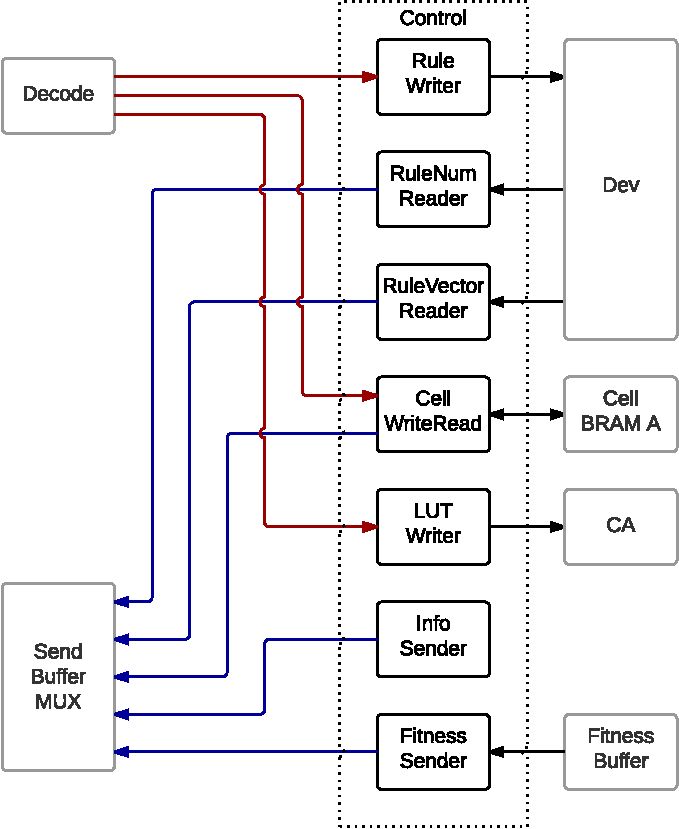
\includegraphics[width=0.7\textwidth]{implementation-control}
    \caption[Control modules]{
        Detailed block diagram of the Control modules.
        Red signals are inputs while blue are outputs.
        Control signals are not shown.
    }
    \label{fig:implementation-control}
\end{figure}

Below are details about the different modules, in order of increasing complexity.
\todo{rewrite/remove this?}
\todo{send to system = put into transmission buffer}
\todo{possible to create deadlocks due to waiting}

\subsection{Rule Writer}

The purpose of the Rule Writer is to store new rules to the Rule BRAM within the Development module.
It is, along with the LUT Writer, the simplest control module.
When activated, it stores one rule to a specified index of the Rule BRAM.
The index doubles as priority for a rule, with higher indexes having higher priority.

As explained in Section~\ref{sec:development}, index zero is reserved for representing that no rules have triggered.
Writing a rule to it has no effect as the rule testers are reset instead of testing the rule during development.

\subsection{LUT Writer}

The purpose of the LUT Writer is to store new LUTs to the LUT BRAM within the Cellular Automaton module.
It is, along with the Rule Writer, the simplest control module.
When activated, it stores one LUT to a specified index of the LUT BRAM.
The index signifies the cell type that should be converted into the LUT.
\todo{clarify}

\subsection{Information Sender}

Nearly all parts of the system are parameterized.
The previous practice of manually ensuring that the parameters of both the design and API were in sync was both tiresome and prone to error.
Therefore, the Information Sender provides a means for the API to automaticly query these parameters.

When activated, it puts all parameters that might be useful into the the Transmission Buffer.
This includes information about the CA such as the size, whether wrapping is enabled, and number of bits per state and type;
information about counters available for control flow;
maximum number of rules;
and information about the fitness modules, such as the type and output size.

\subsection{Fitness Sender}

The Fitness Sender is responsible for sending the output of the Fitness module to the host.
As this is data is stored in the Fitness Buffer, is is a simple matter of moving it to the Transmission Buffer when the data is available and the buffer is ready.
As described in Section~\ref{sec:fitness}, the Fitness module declares how many words should be sent per output value.
This is taken into account by the Fitness Sender when activated.
\todo{do something with last sentence}

\subsection{Rule Vector Reader}

The Rule Vector Reader is tasked with reading the rule vectors created by the Development module and sending them to the host.
Multiple rule vectors can be read with one instruction.
Since rule vectors can be of any length, they are each split over multiple words, starting with the lowest indexes.
The final word of each vector is padded with zeroes.
\todo{this sentence is a bit off}
For more information on rule vectors, see Section~\ref{sec:development}.

\subsection{Rule Numbers Reader}
\label{sec:rule-numbers-reader}

The Rule Numbers Reader is tasked with reading each cell's most recently activated development rule and sending them to the host.
The rule numbers are stored in the Rule Numbers BRAM of the Development module and are scanned in raster order\footnotemark.
\footnotetext{
    In raster scanning, two-dimensional data is read line-by-line, least significant to most significant.
    This is extendable to 3D; first X is incremented, then Y, then Z.
    \todo{better explanation}
}

Each word is fitted with as many rule numbers as possible without splitting them over multiple words or containing ones from different rows.
Any remaining space is filled with zeroes.
\todo{more details?}

\subsection{Cell Writer Reader}

The purpose of the Cell Writer Reader is to perform read and write operations against Cell BRAM A, causing it to be the system's main input/output channel.
It is possible to write states and types to either a single cell, a row of cells or the entire BRAM, while it it is possible to read from a single cell or the entire BRAM.

It is easily the most complex control module, due to the intricate operations required to change only selected values in BRAM rows.
Additionally, it must convert variable-width types and states into fixed-width words in an efficient manner when reading.

The module consists of combiners which are used to combine new data with existing data from the Cell BRAM, repeaters to simplify the process of filling the entire Cell BRAM with a given state and type, shifters used to select output, and a state machine which controls everything.
\figurename~\ref{fig:implementation-cell-writer-reader} shows how the components are connected.

\begin{figure}[!ht]
    \centering
    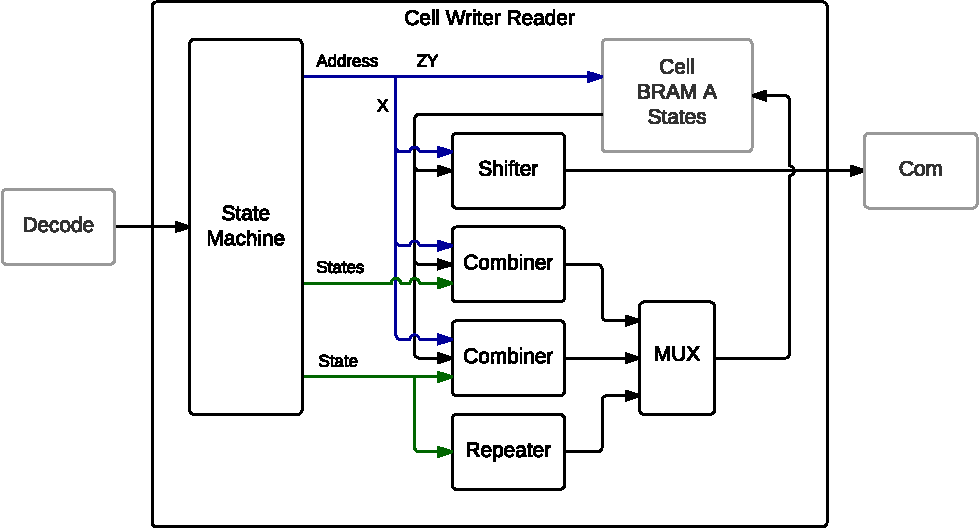
\includegraphics[width=\textwidth]{implementation-cell-writer-reader}
    \caption[Cell Writer Reader]{
        Detailed block diagram of the Cell Writer Reader.
        Only the state part is shown to reduce complexity; the type part is identical.
        Cell BRAM A is drawn inside the module for completeness.
        Control signals are not shown.
    }
    \label{fig:implementation-cell-writer-reader}
\end{figure}

\subsubsection{Combiner}

The combiner is a combinatorial unit that combines two signals of different lengths by replacing one part of the long signal with the short signal.
This is implemented using a shifter and a mask that is the size of the short signal.
First, the short input and mask is shifted into the desired position.
Then, the long signal is anded with the inverted mask and ored with the short signal, producing the combined signal.
The process is illustrated in \figurename~\ref{fig:combiner}.

\begin{figure}[!ht]
    \centering
    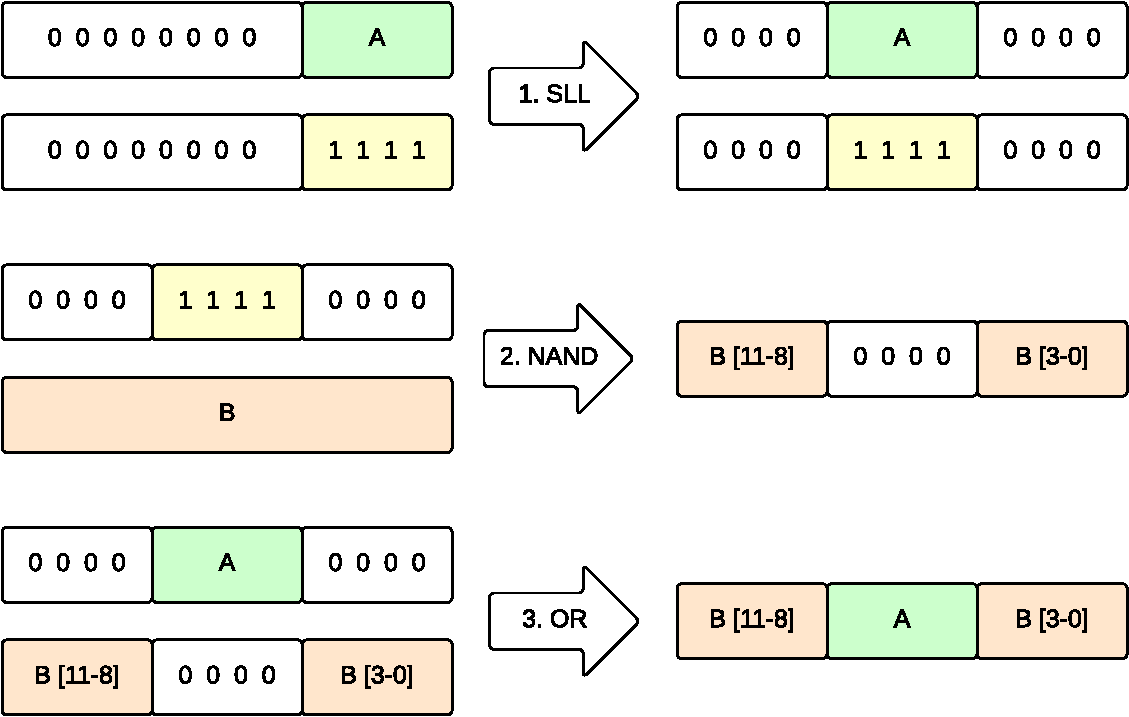
\includegraphics[width=0.8\textwidth]{combiner}
    \caption[Combiner operation]{
        The three operations that power the combiner.
        A is the short input, highlighted in green.
        B is the long input, highlighted in orange.
        The mask is highlighted in yellow.
    }
    \label{fig:combiner}
\end{figure}

\subsubsection{State Machine}

The state machine consists of seven states, shown in \figurename~\ref{fig:statemachine-cell-writer-reader}.
When an operation is received, the BRAM address is set and it transitions from idle to the corresponding state.
Some states are dual-purpose due to the similarity of the operations, while others are not.
Coincidentally, the dual-purpose states complete in one cycle while the others require multiple\footnotemark.
\footnotetext{
    Techically, the Send One state does not necessarily complete in one cycle since it will wait until there is available space in the Transmission Buffer.
    However, it is the common case.
}

\begin{figure}[!ht]
    \centering
    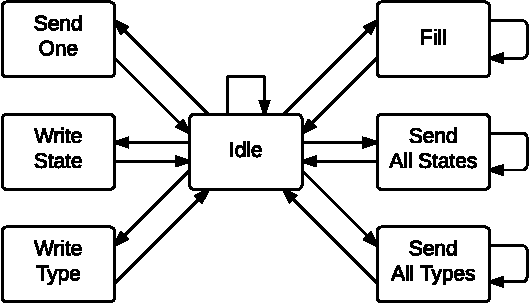
\includegraphics[width=0.55\textwidth]{statemachine-cell-writer-reader}
    \caption{Cell Writer Reader state machine}
    \label{fig:statemachine-cell-writer-reader}
\end{figure}

The dual-purpose states are as follows:
Send One can send either a state or a type, Write State can write either one or a row of states, and Write Type can write either one or a row of types.
The remaining states are:
Fill writes the same state and type to all cells, Send All States reads all states in raster order, and Send All Types reads all types in raster order.
The output formatting of the Send All states is equal to that of the Rule Numbers Reader, detailed in Section~\ref{sec:rule-numbers-reader}.

%==============================================================================%

\section{Cell Storage}

\todo{Buffer -> Storage}

The Cell Storage serves as the location for exchange of cell data between the CA, Development and Host.
It contains two separate storage areas, the contents of which can be swapped.
Each storage area can host a full matrix of cell states and types, and allows one row of each to be read each cycle.
The main reason two storage areas are needed is the Development module.
It requires a place to store its output without affecting its input during the development process.
More on this in Section~\ref{sec:development}.

The module is implemented as two dual-port BRAMs, one for states and one for types, each sized to twice the size of the matrix.
To create two separate storage areas (A and B) with both states and types, the address of the first port is prefixed with 0 and the second with 1.
The contents of the storage areas can then be made to appear swapped by simply inverting the prefix bits.

To service all \todo{word} components, the Cell Storage is connected via a multiplexer.
It has two modes; normal and development.
In normal mode, storage A is connected to the Cell Writer Reader and storage B to the CA.
In development mode, both storage areas are connected to the Development module.

\todo{fig?}

%==============================================================================%

\section{Development}
\label{sec:development}

The Development Module is responsible for providing the ontogenic aspect of the system by allowing cells to be changed based on user-supplied development rules.

\todo{overall implementation}.
It is implemented as an interlocked two-stage pipeline controlled by a statemachine.
Fetch neighborhood, test all rules, writeback.
Pipeline-in-pipeline.
\figurename~\ref{fig:implementation-development}.

\begin{figure}[!ht]
    \centering
    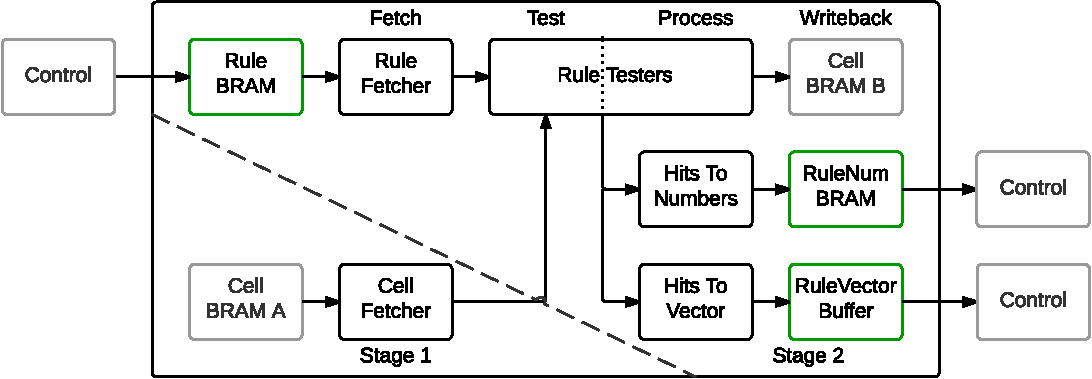
\includegraphics[width=\textwidth]{implementation-development}
    \caption[Development module]{
        Detailed block diagram of the Development module.
        The two main pipeline stages are separated by a dashed line,
        while the substages of the pipeline within the second main stage are marked at the top.
        The cell BRAMs are drawn inside the module for pipeline completeness.
        Control signals are not shown.
    }
    \label{fig:implementation-development}
\end{figure}

Controlled by state machine \figurename~\ref{fig:statemachine-development}.

\begin{figure}[!ht]
    \centering
    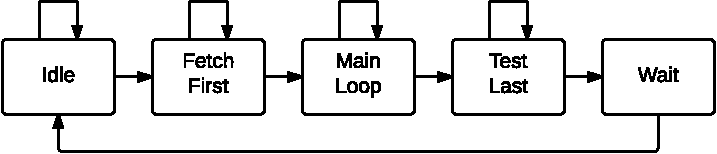
\includegraphics[width=0.75\textwidth]{statemachine-development}
    \caption[Development module state machine]{
        State machine controlling the Development module.
    }
    \label{fig:statemachine-development}
\end{figure}

\subsection{Cell Fetcher}

The first stage is CellFetch, which reads the cell neighborhoods for one row of cells per run.
From Cell Storage A.
\todo{explain access pattern}
This takes 3 cycles for 2D and 5 for 3D.
\figurename~\ref{fig:statemachine-cell-fetcher}.
\todo{CellFetch limiting factor for very few rules}

\begin{figure}[!ht]
    \centering
    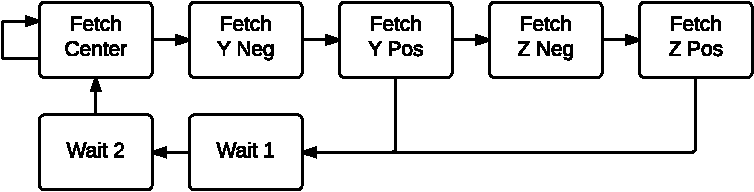
\includegraphics[width=0.8\textwidth]{statemachine-cell-fetcher}
    \caption[Cell Fetcher state machine]{
        State machine for the Cell Fetcher.
    }
    \label{fig:statemachine-cell-fetcher}
\end{figure}

\subsection{Rule Fetcher}

\TODO
One rule ahead to save cycle.
The number of active rules can be set at runtime to reduce development time by skipping unused rules.
Rules are fetched from RuleBRAM, then rules and cell neighborhoods are sent to the RuleTesters.

\subsection{Rule Testers}

\TODO
Rule 0 reserved.
To allow multiple rules to be tested each cycle, RuleTesters is split into two parts.
The first part tests the different rules against each cell, while the second selects the result from the highest priority rule.
After the first part, hits are output from RuleTesters to HitsToVector and HitsToNumbers.
To Cell Storage B.

\subsection{Hits to Numbers}

\TODO
Writes last triggered rule to each cell.

\subsection{Hits to Vector}

Rule vectors are only stored after the final rules and cells.
All triggered rules are written to RuleVectorBuffer (even overridden)
\todo{vectors overwritten to allow development without reading them}

%==============================================================================%

\section{Cellular Automata}

The Cellular Automata module is responsible for configuring the sblock matrix with data from the Cell Buffer, step the sblocks and store the number of live cells, and read the new states back into the Cell Buffer.

It is implemented as a state machine that is manipulating a matrix of sblocks connected to an adder tree.
The adder tree is used to calculate the number of live cells after each step.
The numbers are then stored in the Live Count Buffer.
If the Live Count Buffer is full, data is overwritten, possibly corrupting fitness evaluation, until the buffers are reset.
This design decision was made to allow the CA to run without being required to read fitness data.

When configuring the sblock matrix, cell types are used as an index for the LUTBRAM to find the corresponding LUT entry.

\begin{figure}[!ht]
    \centering
    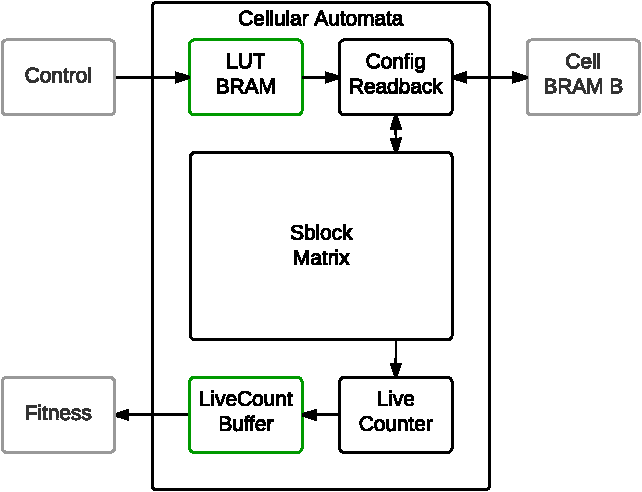
\includegraphics[width=0.7\textwidth]{implementation-cellular-automata}
    \caption[Cellular Automata]{
        Detailed block diagram of the Cellular Automata.
    }
    \label{fig:implementation-cellular-automata}
\end{figure}

\begin{figure}[!ht]
    \centering
    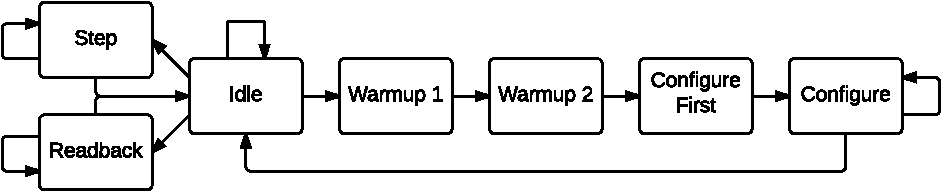
\includegraphics[width=\textwidth]{statemachine-cellular-automata}
    \caption[Cellular Automata state machine]{
        State machine controlling the Cellular Automata.
    }
    \label{fig:statemachine-cellular-automata}
\end{figure}

\begin{itemize}
    \item ConfigReadback is not separate module, but statemachine in CA
\end{itemize}

%==============================================================================%

\section{Fitness}
\label{sec:fitness}

\begin{itemize}
    \item Dataflow-ish (livecountbuffer to fitnessbuffer)
    \item Custom implementation, simple interface
\end{itemize}

\subsection{Live Count}

\todo{simply copies from Live Count Buffer to Fitness Buffer}

\subsection{Discrete Fourier Transform}

\begin{itemize}
    \item Revised version of Ola Martin's
    \item More customizable (describe parameters)
    \item Copies Data to internal buffer, since FIFO is delete-on-read (fig)
\end{itemize}

%==============================================================================%

\section{Software API}

\TODO

\subsection{Communication}

The communication part of the new software API is split into two parts:
\todo{this lone sentence is kinda awkward}

The first is a general interface for connecting to PCI and PCI Express devices without using a custom driver.
It takes advantage of Linux' automatic population of /sys/devices/pci* with files representing the memory regions of all PCI and PCI Express devices.
The directory is searched by vendor and device id, and the corresponding memory regions is memory-mapped into the program.

The second is an interface specifically for the communication unit.
It provides open, close, read and write functions similar to the old BenERA interface, in addition to implementing all special request functions in Table~\ref{tab:requests}.
When a read or write operation is initiated, buffers are checked for available data or space.
If there is not enough present, the program waits and then rechecks.

%==============================================================================%

\todo{where? also tweak language}
By default, neighbors which would be outside the matrix are treated as having a state and type of zero.
However, when matrix wrap is enabled, neighbors on the opposite side of the matrix are used instead.
This applies to both runstep and devstep.
